\newif\ifshowsolutions
\showsolutionsfalse
\documentclass{article}
\usepackage{listings}
\usepackage{amsmath}
\usepackage{subfig}
\usepackage{amsthm}
\usepackage{amsmath}
\usepackage{amssymb}
\usepackage{graphicx}
\usepackage{mdwlist}
\usepackage{geometry}
\usepackage{titlesec}
\usepackage{palatino}
\usepackage{mathpazo}
\usepackage{fancyhdr}
\usepackage{paralist}
\usepackage{todonotes}
\usepackage{tikz}
\usepackage{float} % Place figures where you ACTUALLY want it
\usepackage{comment} % A hack to toggle sections
\usepackage{ifthen}
\usepackage{mdframed}
\usepackage{verbatim}
\usepackage{listings}
\usepackage{bbm}
\usepackage{upquote} % Prevents backticks replacing single-quotes in verbatim
\usepackage{listings}
\lstset{basicstyle=\ttfamily,
  showstringspaces=false,
  commentstyle=\color{red},
  keywordstyle=\color{blue}
}
\usepackage[strings]{underscore}
\usepackage[colorlinks=true]{hyperref}
\usetikzlibrary{positioning,shapes,backgrounds}

\geometry{margin=1in}
\geometry{headheight=2in}
\geometry{top=2in}

\setlength{\marginparwidth}{2.15cm}
\setlength{\parindent}{0em}
\setlength{\parskip}{0.6\baselineskip}

\rhead{}
\lhead{}

% Spacing settings.
\titlespacing\section{0pt}{12pt plus 2pt minus 2pt}{0pt plus 2pt minus 2pt}
\titlespacing\subsection{0pt}{12pt plus 4pt minus 2pt}{0pt plus 2pt minus 2pt}
\titlespacing\subsubsection{0pt}{12pt plus 4pt minus 2pt}{0pt plus 2pt minus 2pt}
\renewcommand{\baselinestretch}{1.15}

% Shortcuts for commonly used operators.
\newcommand{\E}{\mathbb{E}}
\newcommand{\Var}{\operatorname{Var}}
\newcommand{\Cov}{\operatorname{Cov}}
\newcommand{\Bias}{\operatorname{Bias}}
\DeclareMathOperator{\argmin}{arg\,min}
\DeclareMathOperator{\argmax}{arg\,max}

% Do not number subsections and below.
\setcounter{secnumdepth}{1}

% Custom format subsection.
\titleformat*{\subsection}{\large\bfseries}

% Set up the problem environment.
\newcounter{problem}[section]
\newenvironment{problem}[1][]
{\begingroup
  \setlength{\parskip}{0em}
  \refstepcounter{problem}\par\addvspace{1em}\textbf{Problem~\Alph{problem}\!
    \ifthenelse{\equal{#1}{}}{}{ [#1 points]}:}
  \endgroup}

% Set up the subproblem environment.
\newcounter{subproblem}[problem]
\newenvironment{subproblem}[1][]
{\begingroup
  \setlength{\parskip}{0em}
  \refstepcounter{subproblem}\par\medskip\textbf{\roman{subproblem}.\!
    \ifthenelse{\equal{#1}{}}{}{ [#1 points]:}}
  \endgroup}

% Set up the teachers and materials commands.
\newcommand\teachers[1]
{\begingroup
  \setlength{\parskip}{0em}
  \vspace{0.3em} \textit{\hspace*{2em} TAs responsible: #1} \par
  \endgroup}
\newcommand\materials[1]
{\begingroup
  \setlength{\parskip}{0em}
  \textit{\hspace*{2em} Relevant materials: #1} \par \vspace{1em}
  \endgroup}

% Set up the hint environment.
\newenvironment{hint}[1][]
{\begin{em}\textbf{Hint: }}
    {\end{em}}


% Set up the solution environment.
\ifshowsolutions
  \newenvironment{solution}[1][]
  {\par\medskip \begin{mdframed}\textbf{Solution~\Alph{problem}#1:} \begin{em}}
        {\end{em}\medskip\end{mdframed}\medskip}
  \newenvironment{subsolution}[1][]
  {\par\medskip \begin{mdframed}\textbf{Solution~\Alph{problem}#1.\roman{subproblem}:} \begin{em}}
        {\end{em}\medskip\end{mdframed}\medskip}
\else
  \excludecomment{solution}
  \excludecomment{subsolution}
\fi


\chead{
  {\vbox{
      \vspace{2mm}
      \large
      Computational Physics II \hfill
      UCSD PHYS 142/242 \hfill \\[1pt]
      Assignment 2\hfill
      Draft version due: Friday, February 9, 2024, 8:00pm\\
	  \hfill
	  Corrected version due: Wednesday, February 14, 2024, 8:00pm\\
    }
  }
}

\begin{document}
\pagestyle{fancy}

\section*{Policies}
\begin{itemize}
  \item You are free to collaborate on all of the problems, subject to the collaboration policy stated in the syllabus.
  \item You should submit all code used in the homework.
        You are free to use Python, C/C++, Julia, or any other code \textbf{within reason} as long as you comment your code such that the TA can follow along and run it without any issues.
\end{itemize}

\section*{Submission Instructions}
\textbf{PLEASE NOTE} that there are two steps to submitting your Homework.
Both must be submitted by the deadline.

\begin{itemize}
  \item Please submit your report as a single .pdf file to Gradescope under ``Assignment 2 Draft" or ``Assignment 2 Corrections".
        \textbf{In the report, include any images generated by your code along with your answers to the questions.}
        For instructions specifically pertaining to the Gradescope submission process, see \url{https://www.gradescope.com/get_started#student-submission}.
  \item Please submit your code as a .zip archive to Gradescope under ``Assignment 2 Code Draft'' or ``Assignment 2 Code Corrections".
        The .zip file should contain all of your source code files.
\end{itemize}

\newpage
\section{Tunneling in the Double Potential Well [40 Points]}
\materials{Week 4 lectures}

Consider the double potential well,
\begin{equation}
  V(x) =  \alpha x^4  - 2x^2 + + \frac{1}{\alpha}
\end{equation}
where $x$ is the position of the particle, and we set $m=\hbar=1$.
For parts 1A, 1B, and 1C, you may set $\alpha = 0.4$.
For the last part, you will need to vary $\alpha$.
The minima of the potential are at $x_\mathrm{min}^2 = \pm\frac{1}{\alpha}$ and the barrier height is $V(0) = \frac{1}{\alpha}$.
The potential is shown in the figure below.
\begin{center}
  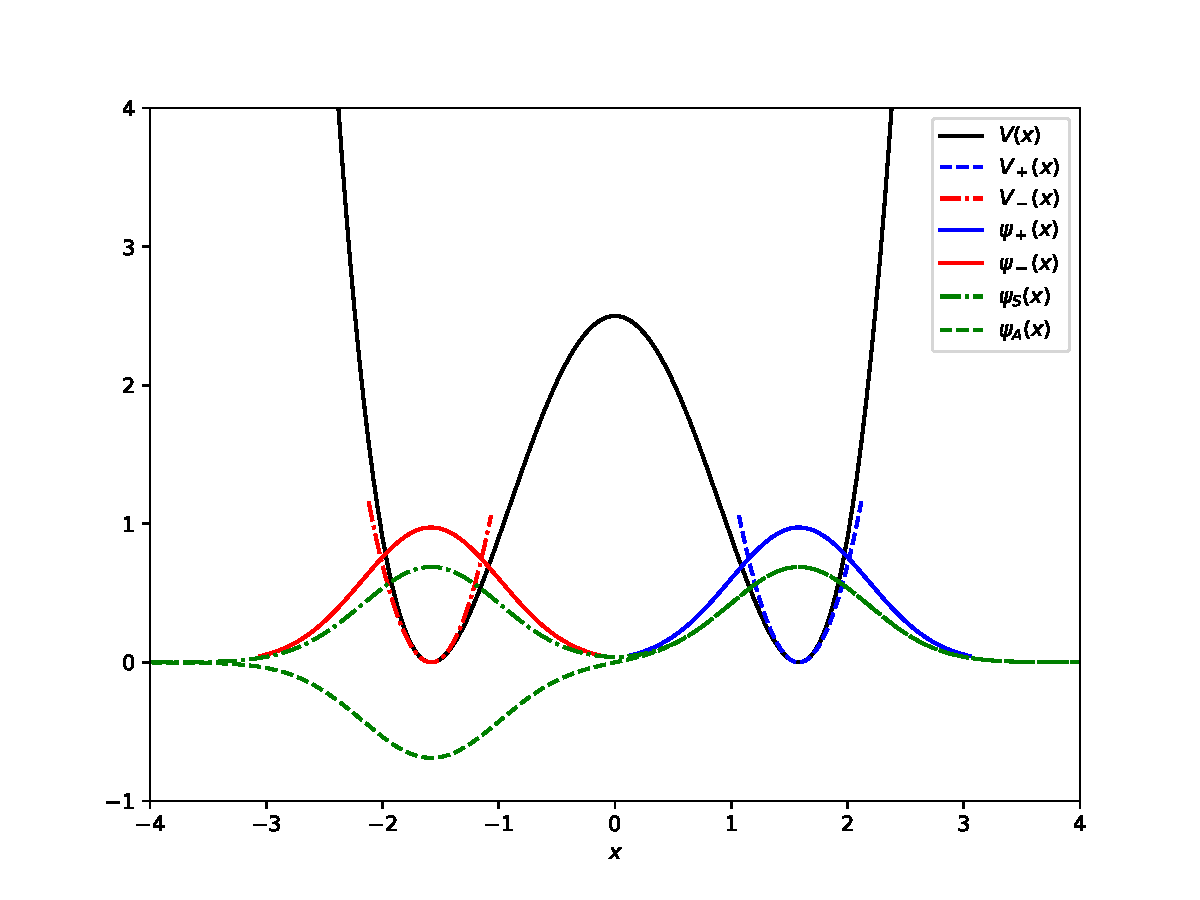
\includegraphics[width=0.5\textwidth]{V_all.pdf}
\end{center}

As discussed in lecture 9, we can approximate the potential by a harmonic potential near the minima.
\begin{align}
  V_+(x) & = 4(x-x_\mathrm{min})^2  \\
  V_-(x) & = 4(x+x_\mathrm{min})^2,
\end{align}
which implies $\omega = 2\sqrt{2}$.
The ground state wave functions for those approximate potential wells are
\begin{align}
  \psi_+(x) & = \left(\frac{\omega}{\pi}\right)^{1/4} \exp\left(- \frac{\omega}{2}(x-x_\mathrm{min})^2\right) \\
  \psi_-(x) & = \left(\frac{\omega}{\pi}\right)^{1/4} \exp\left(- \frac{\omega}{2}(x+x_\mathrm{min})^2\right)
\end{align}
We can approximate the ground state and first excited state as the symmetric and antisymmetric combinations of these wave functions, respectively.
\begin{align}
  \psi_0(x) & \approx \psi_\mathrm{S}(x) = \frac{1}{\sqrt{2}}\left ( \psi_+(x) + \psi_-(x) \right ) \\
  \psi_1(x) & \approx \psi_\mathrm{A}(x) = \frac{1}{\sqrt{2}}\left ( \psi_+(x) - \psi_-(x) \right )
\end{align}
The energy gap between the ground state and first excited state is $\Delta E = E_1 - E_0$.

\begin{problem}[10]
Demonstrate tunneling between the two wells using the Feynman path integral.
Start with the particle in the right well
\begin{equation}
  \psi(x, 0) = \psi_+(x),
\end{equation}
and evolve the wave function at each time step using the elementary propagator.

Numerically, you may use discretization parameters similar to Assignment 1: $\epsilon = \Delta t = \pi/128$, $x_0 = -4$, $x_{N_D} = +4$, and $N_D=600$.
You will have to simulate a long enough period $T > t_\mathrm{tunnel}$ that is longer than the tunneling time.
As a reminder, the tunneling time is defined as the time it takes for the particle to reach the left well.

Plot the mean position $\langle x \rangle$ as a function of time $t$.
How can you estimate the tunneling time $t_\mathrm{tunnel}$ from this plot?

\begin{hint}
  You may approximate the propagator as
  \begin{equation}
    \tilde {\mathcal K}(x_b, \epsilon; x_a, 0) \sim \exp \left( i \left(\frac{1}{2}\frac{(x_b - x_a)^2}{\epsilon} - V\left(\frac{x_a+x_b}{2}\right) \epsilon\right) \right),
  \end{equation}
  where $x_a$ and $x_b$ are the initial and final positions, respectively, and $\epsilon$ is the time step.
  Note, we lack the normalization factor in this approximation so you will need to normalize the wave function at each time step
  \begin{equation}
    \psi(x, t) \leftarrow \frac{\psi(x, t)}{\sqrt{\int_{-\infty}^{\infty} |\psi(x, t)|^2 dx}}.
  \end{equation}
\end{hint}
\end{problem}

\begin{solution}
\end{solution}

\begin{problem}[10]
Estimate the energy gap $\Delta E$ between the ground state and first excited state.

\begin{hint}
  To estimate $E_0$ and $E_1$, you can use the expectation value of the Hamiltonian operator,
  \begin{align}
    E_0 & \approx \int \psi_\mathrm{S}^*(x) \hat H \psi_\mathrm{S}(x) dx, \\
    E_1 & \approx \int \psi_\mathrm{A}^*(x) \hat H \psi_\mathrm{A}(x) dx,
  \end{align}
  where $\hat H = -\frac{1}{2}\frac{\partial^2}{\partial x^2} + V(x)$.
  This method may not agree with the numerical result shared in lecture 9.
\end{hint}
\end{problem}

\begin{solution}
\end{solution}

\begin{problem}[10]
Animate the evolution of the real and imaginary parts of the wave function $\psi(x, t)$ and the probability $|\psi(x, t)|^2$ as a function of time $t$ over a period $T > t_\mathrm{tunnel}$ and save it as a \texttt{.gif} or \texttt{.mp4} file.
\end{problem}

\begin{solution}
\end{solution}

\begin{problem}[10]
Determine an approximate relationship between the tunneling time $t_\mathrm{tunnel}$ and the energy gap $\Delta E$ between the ground state and first excited state.

\begin{hint}
  Vary $\alpha$ and calculate the energy gap $\Delta E$ and tunneling time $t_\mathrm{tunnel}$ for each $\alpha$ as you did in parts 1A and 1B.
\end{hint}

\end{problem}

\begin{solution}
\end{solution}

\end{document}
